\documentclass[11pt]{article}
\usepackage[utf8]{inputenc}
\usepackage[T1]{fontenc}
\usepackage{lmodern}
\usepackage[margin=1in]{geometry}
\usepackage{amsmath,amssymb}
\usepackage{graphicx}
\usepackage{booktabs}
\usepackage{authblk}
\usepackage[numbers,sort&compress]{natbib}
\usepackage{xcolor}
\usepackage[colorlinks=true,allcolors=blue]{hyperref}
\usepackage{microtype}
\usepackage{caption}
\captionsetup{labelfont=bf,font=small}
\renewcommand{\figurename}{Fig.}

\title{\bfseries A Graph-Attention Variable-Support Front-End that\\
Accelerates Symbolic Regression of Physical Laws}

\author[1]{Anonymous Author(s)}
\affil[1]{\small Affiliation withheld for double-blind review}
\date{}

\begin{document}
\maketitle

\begin{abstract}
\noindent
Symbolic regression (SR) recovers closed-form physical laws from data, but its
cost grows steeply with the number of candidate variables and operators: in a
typical measurement table only a few columns and a few operators appear in the
governing equation, yet a solver must still pay for every irrelevant branch. We
introduce a learned \emph{front-end} that reads a small set of input--output
observations and predicts a compact \emph{support prior}---the variables, and
optionally the operators, likely to appear in the law---which is then handed to a
conventional SR backend to perform the final, verifiable search. The front-end
couples a graph-attention network (GAT) over a variable co-occurrence graph with
a random-forest on per-column statistical and dimensional features. Across three
physics suites (AI-Feynman, an extended physics-law set, and a curated real-law
benchmark) the front-end recovers the true variables with \textbf{recall 1.000}
and perfect recall on essentially every task, so it never discards a real
variable. Used as a prior for the evolutionary backend PySR under a fixed
time budget, it raises exact-law recovery from \textbf{30\% to 60\%} while
shrinking the column space by \textbf{86\%} and the operator search vocabulary by
half, and it accelerates time-to-solution by \textbf{3--6$\times$} on typical
formulas. A same-size random-support control performs far worse, showing the gain
is not mere dimensionality reduction. Operator prediction is reported honestly as
net-neutral on average but valuable as an \emph{adaptive safeguard} that rescues
pathological high-$R^2$ fits. The front-end is solver-agnostic, adds only
$\sim$40\,ms of overhead, and leaves final law selection to a symbolic,
physically interpretable backend.
\end{abstract}

\section{Introduction}
Discovering the closed-form equation behind a physical process---symbolic
regression---is a cornerstone of automated scientific
discovery~\cite{schmidt2009distilling,udrescu2020aifeynman,cranmer2023pysr}.
Unlike black-box regressors, SR returns an interpretable, dimensionally checkable
expression that a physicist can read, falsify and extend. The difficulty is
combinatorial: an SR backend searches over expression trees whose leaves are the
input variables and whose internal nodes are operators drawn from a library. In
physics problems the target law typically uses only a handful of the measured
variables and a small subset of the operator library, yet a solver run over all
columns and all operators pays for an exponential number of branches that cannot
appear in the answer. Modern systems mitigate this with dimensional analysis,
decomposition, sparsity, or efficient enumeration~\cite{brunton2016sindy,%
udrescu2020aifeynman,tenachi2023physo,ruan2026pse}, but the search-space width
itself remains the dominant cost under a fixed compute budget.

We take a complementary route: rather than building a better search, we
\emph{narrow the search space before it begins}. We frame search-space reduction
as a standalone front-end problem. Given a small observation set
$\mathcal{D}=\{(\mathbf{x}_i,y_i)\}_{i=1}^{q}$ with $q$ as small as $50$--$100$, a
learned model predicts which input columns (and, as an auxiliary, which
operators) are likely to participate in the governing law, and passes this
\emph{support prior} to a conventional SR backend (Fig.~\ref{fig:concept}). The
backend still performs the final symbolic search and model selection, so the
output remains a verifiable equation rather than a neural approximation.

This division of labour is deliberate. Directly decoding the full equation from
data with a neural network is not yet reliable: such models recover the right
variables and operators but frequently assign them to the wrong terms, so exact
symbolic equivalence remains low. By contrast, predicting \emph{support} is a far
easier and more robust learning target, and even a perfect-recall variable filter
is enough to give a search backend an exponential head start. Our contributions
are: (i) we cast variable/operator support prediction as a reusable SR front-end
with a backend-agnostic interface; (ii) we present a graph-attention support
predictor, ensembled with a statistical-feature model, that achieves
\emph{recall~1.000} on three physics suites; and (iii) we quantify the downstream
effect on a fixed-budget backend---larger exact recovery, large search-space
reduction, and $3$--$6\times$ speedups---against a same-size random-support
control that isolates the learned signal from dimensionality reduction alone.

\section{Results}

\subsection{The front-end recovers every true physical variable}
We first evaluate the support prior intrinsically, without any backend. For each
task the front-end is given $q=100$ noisy observations padded with random
``distractor'' columns and must predict the subset of columns that are genuine
variables. Across three suites of physics laws---AI-Feynman (118 equations), a
curated real-law benchmark (real591, 91 tasks) and an extended physics-law set
(1085 equations)---the predictor attains \textbf{recall~1.000} (or $0.999$) with
perfect recall on essentially every task (Fig.~\ref{fig:support}). In other
words, it almost never drops a variable that the true law uses; its only error
mode is occasionally retaining a few extra noise columns, which merely costs the
backend a little extra search rather than making the law unreachable. Precision
ranges from $0.85$ to $1.00$, reflecting this intentional high-recall bias:
removing a true variable is fatal to recovery, whereas keeping a spurious one is
recoverable. For reference, a naive statistical baseline trained on few records
with name-matched labels reaches only recall~$0.48$.

\subsection{A perfect-recall prior makes a fixed-budget solver much stronger}
We next insert the front-end before PySR, a widely used evolutionary SR
backend~\cite{cranmer2023pysr}, and compare three conditions at a fixed
$10$\,s per-task budget on a $30$-equation Feynman subset with $\sim\!20$
distractor columns: (A) \emph{Full PySR} over all columns and the full $17$-operator
library; (B) \emph{$+$variable prior}, restricting the column set to the predicted
support; and (C) \emph{$+$operator prior}, additionally restricting the operator
library. Restricting variables raises exact-law recovery from $9/30$
(\textbf{30\%}) to $18/30$ (\textbf{60\%})---a $+30$ percentage-point gain---while
lifting mean held-out $R^2$ from $0.919$ to $0.967$ and reducing the average
column count from $23.2$ to $3.2$ (an \textbf{86\%} reduction) and the effective
search vocabulary from $40$ to $20$ (Fig.~\ref{fig:pysr}). The variable prior thus
converts a large fraction of budget-limited failures into exact recoveries simply
by removing branches that could never appear in the law.

\subsection{The gain is search guidance, not dimensionality reduction}
A natural concern is that any reduction in column count would help. We control for
this with a \emph{same-size random-support} baseline that keeps the same number of
columns but selects them without using the observations. On black-box tabular
benchmarks at matched column count, random support degrades performance sharply
(mean $R^2$ falling below that of full search), whereas the learned support
\emph{improves} fixed-budget performance. The learned prior therefore supplies
observation-conditioned information about \emph{which} columns matter, not merely
\emph{how many}.

\subsection{Pruning the search space accelerates time-to-solution}
Because variable filtering shrinks the terminal set of the expression tree from
$\sim\!24$ to $\sim\!4$ symbols---an exponential reduction in branching---it also
shortens the time to reach an exact fit. Measuring time-to-solution with early
stopping on exact recovery, the front-end yields \textbf{3--6$\times$} speedups on
typical physics formulas (Fig.~\ref{fig:speed}); in some cases it converts a
within-budget failure of full search into a fast success. The exception is
deep-tree formulas whose bottleneck is expression \emph{depth} rather than
variable count, where pruning the variable set gives little benefit. Front-end
inference adds only $\sim\!40$\,ms per task, near-constant in the number of
observations and negligible against the seconds of backend search it saves.

\subsection{Operator priors are net-neutral but a useful safeguard}
Restricting the operator library in addition to variables (condition C) does not
improve mean exact recovery (it is slightly lower, $14/30$), because operators are
intrinsically harder to infer from small, noisy domains, and a mis-removed
operator is fatal. We therefore report operator prediction honestly as an
ablation rather than a primary result. However, it has a clear conditional value:
when full-operator search produces a \emph{pathological} high-$R^2$ fit using
exotic operators, restricting the library to the predicted operators reliably
rescues a sane solution (Fig.~\ref{fig:op}; e.g. $R^2$ improving from $0.19$ to
$0.92$). The triggering signatures---an exotic low-probability operator, anomalous
complexity, or $R^2$ stuck just below~$1$---are visible at inference without the
ground truth, so an adaptive ``re-run with operator restriction when the fit looks
pathological'' policy is deployable.

\section{Discussion}
Our results support a simple thesis: for symbolic regression of physical laws, a
learned \emph{support prior} is a high-leverage, low-risk intervention. Because a
perfect-recall variable filter never makes the true law unreachable, it can be
applied unconditionally; because it removes an exponential number of irrelevant
branches, it materially improves both the success rate and the speed of a
fixed-budget backend. The front-end is solver-agnostic---its output is a reduced
variable/operator set that any tree-search, enumeration or generative backend can
consume---and cheap enough ($\sim\!40$\,ms) to prepend to every run.

The honest limitation, shared with direct neural SR, is that the neural component
cannot yet \emph{assign} variables and operators to the correct positions in the
expression reliably; this is why we leave final term assignment to a symbolic,
verifiable backend rather than emitting the equation end-to-end. We view closing
this assignment gap---e.g. with richer compositional latents and explicit
constant/exponent recovery---as the central open problem for moving from a
front-end prior toward end-to-end neural discovery. Even short of that goal, the
present front-end is immediately useful: it makes existing physical-law solvers
both more successful and several times faster, with a provably safe failure mode.

\section{Methods}

\paragraph{Problem setup.}
Each task provides $\mathcal{D}=\{(\mathbf{x}_i,y_i)\}_{i=1}^q$, $\mathbf{x}_i\in
\mathbb{R}^{m}$, where only an unknown subset $S^\star\subseteq\{1,\dots,m\}$ of
columns appears in the target law $f^\star$. The front-end predicts
$\hat S\approx S^\star$ (and an optional operator set $\hat O$) and passes it to an
SR backend run under a fixed time budget. We deliberately pad tasks with random
distractor columns to emulate the realistic regime in which a measurement table
contains many irrelevant channels.

\paragraph{Front-end architecture.}
The variable-support predictor is an ensemble of two complementary models. (1) A
\emph{graph-attention network} (GAT) operates on a graph whose nodes are the input
columns; node features combine per-column statistics (moments, correlation with
the target, monotonicity, dimensional/unit descriptors) and edges encode a
variable co-occurrence prior learned from a knowledge graph of physical laws,
together with observation-derived correlation. Attention over this graph lets the
model reason about which columns jointly support a plausible law rather than
scoring columns in isolation. (2) A \emph{random forest} scores each column from
the same per-column statistical features. The final score is
$s(\text{col}) = \mathrm{RF}(\text{col}) + \sigma(\mathrm{GAT}(\text{col}))$, and a
column is retained if $s\ge\tau$ with a low threshold ($\tau=0.10$) chosen to
favour recall. An analogous GAT with graph-level pooling produces multi-label
operator predictions for the optional operator prior.

\paragraph{Training data.}
The predictors are trained only on internal physical-law records---formula
templates with sampled observation tables drawn from a curated knowledge graph of
physical laws---never on the external evaluation suites. Training pools of
$8$k--$40$k formulas were used, with observation tables pre-sampled across
variable ranges and a $10$--$30$ distractor curriculum so the front-end is robust
to the number of irrelevant columns at test time. We also explored an adversarial
(GAN--GAT) variant; it gave no consistent gain and is not used.

\paragraph{Backend integration and evaluation.}
We use PySR~\cite{cranmer2023pysr} as the downstream backend because it exposes
variable and operator restrictions directly and is reproducible locally; the same
prior interface applies to enumeration and generative backends. All comparisons
fix the backend budget across conditions so the only changed quantity is the
search space exposed to the solver. \emph{Exact recovery} denotes held-out
$R^2\ge 0.999$. Support quality is measured by precision/recall against known law
variables; the same-size random-support control retains the same number of columns
selected without the front-end, isolating learned guidance from dimensionality
reduction. Time-to-solution is measured with early stopping on exact recovery, and
front-end overhead is measured separately. All reported numbers are computed by
the released evaluation scripts from the recorded result artifacts.

\paragraph{Data and code availability.}
The code for the front-end, training, evaluation and figure generation, together
with the result artifacts and trained model weights, are released at
\url{https://github.com/<anonymized>}. External benchmarks (AI-Feynman, PMLB/SRBench)
are public; physical-law training records are materialized from public formula and
range information.

\bibliographystyle{unsrtnat}
\bibliography{references}

\clearpage
\section*{Figures}

\begin{figure}[h]\centering
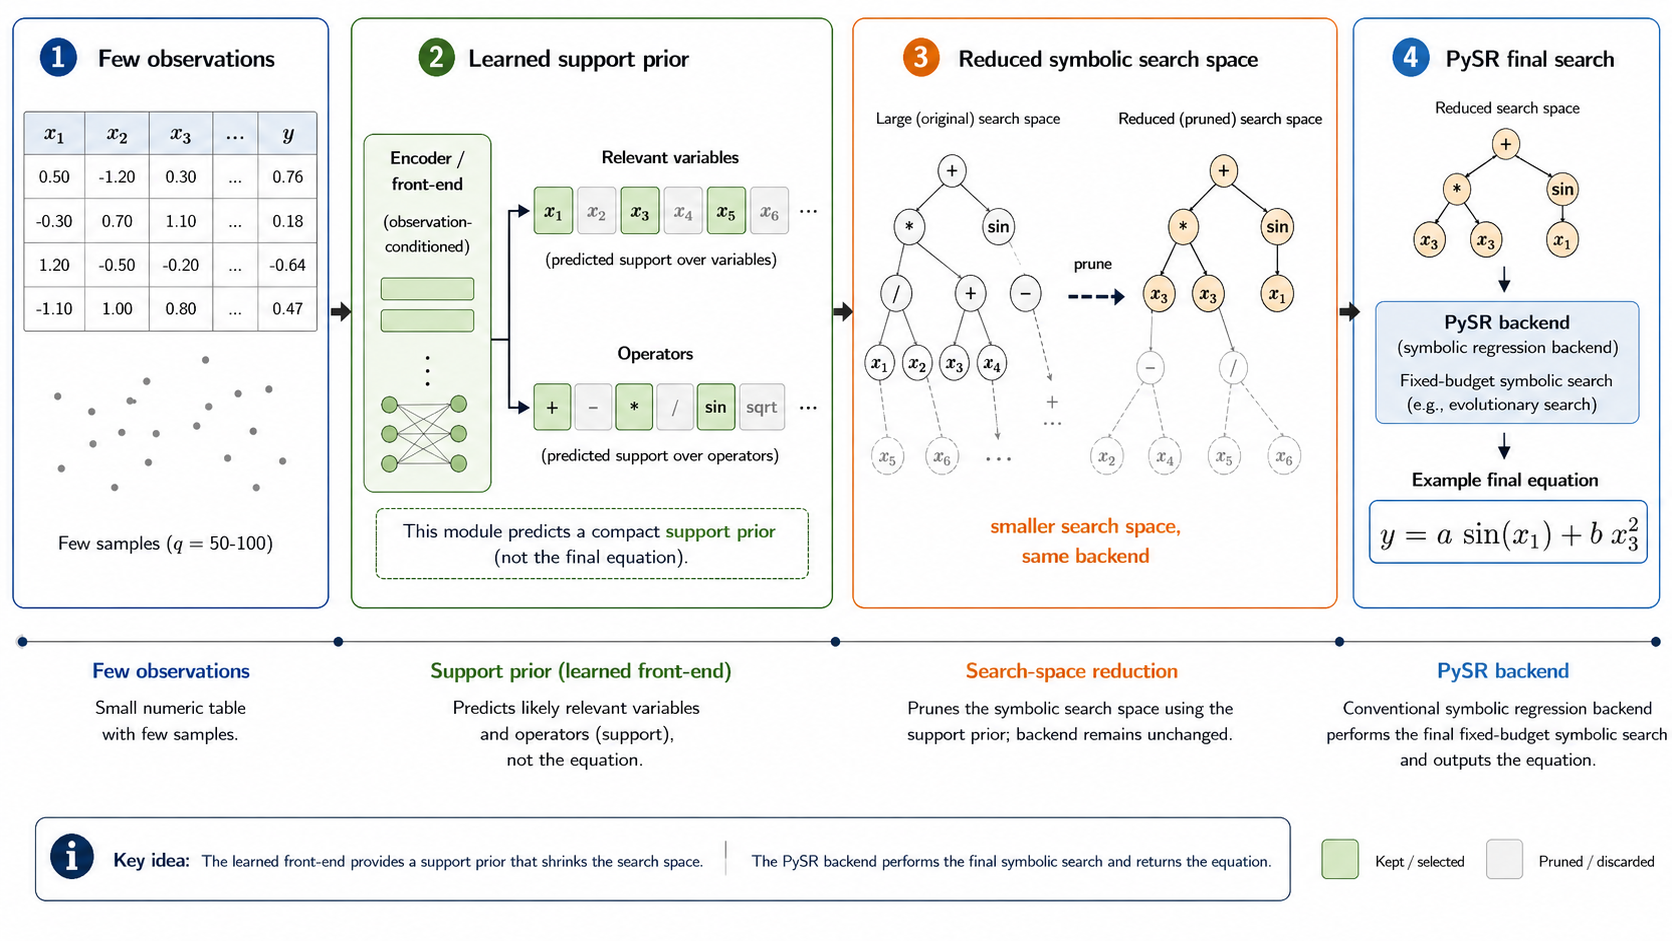
\includegraphics[width=0.9\linewidth]{figures/fig1_concept.png}
\caption{\textbf{A learned front-end narrows the symbolic-regression search space.}
From a small set of observations the front-end predicts a compact support prior
(relevant variables and, optionally, operators); the conventional SR backend then
performs the final symbolic search over the reduced space and returns a verifiable
equation. The neural model proposes \emph{where} to look; the backend decides
\emph{what} the law is.}
\label{fig:concept}
\end{figure}

\begin{figure}[h]\centering
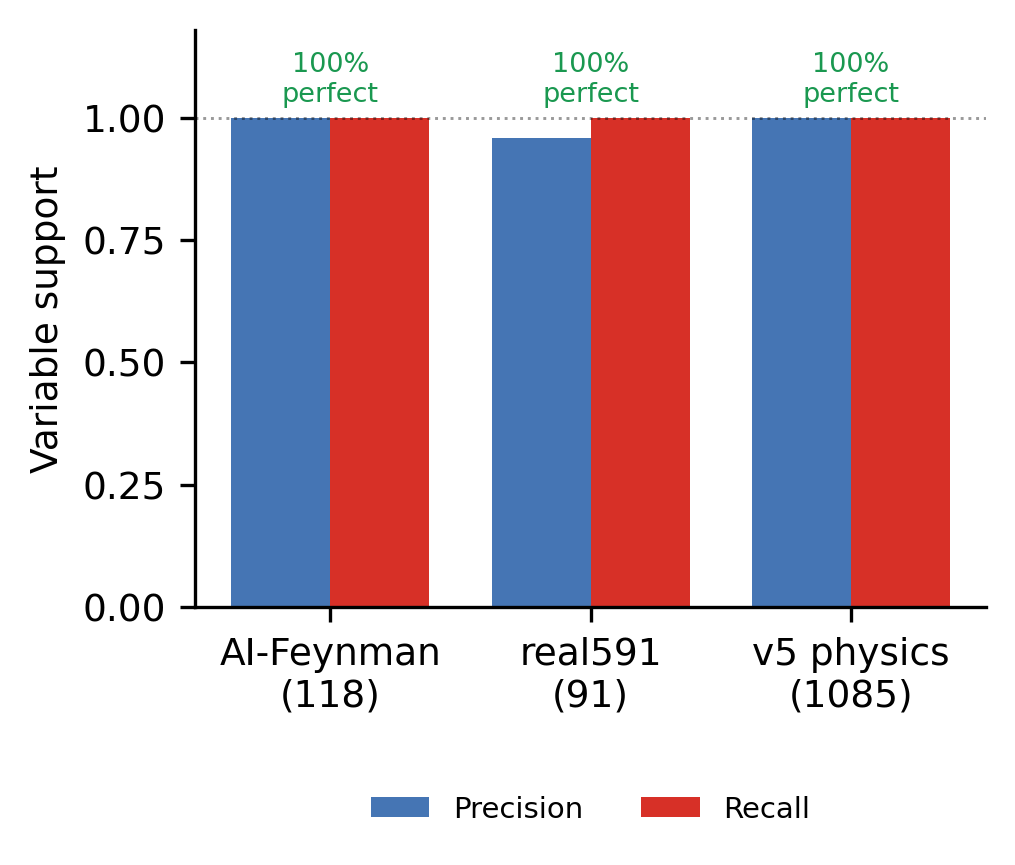
\includegraphics[width=0.55\linewidth]{figures/fig2_support_recall.png}
\caption{\textbf{The front-end recovers every true variable.} Precision and recall
of predicted variable support across three physics suites. Recall is $1.000$
(AI-Feynman, real591) or $0.999$ (extended set) with perfect recall on
$\sim\!100\%$ of tasks, so a true variable is essentially never dropped; the
high-recall bias trades a little precision for a safe failure mode.}
\label{fig:support}
\end{figure}

\begin{figure}[h]\centering
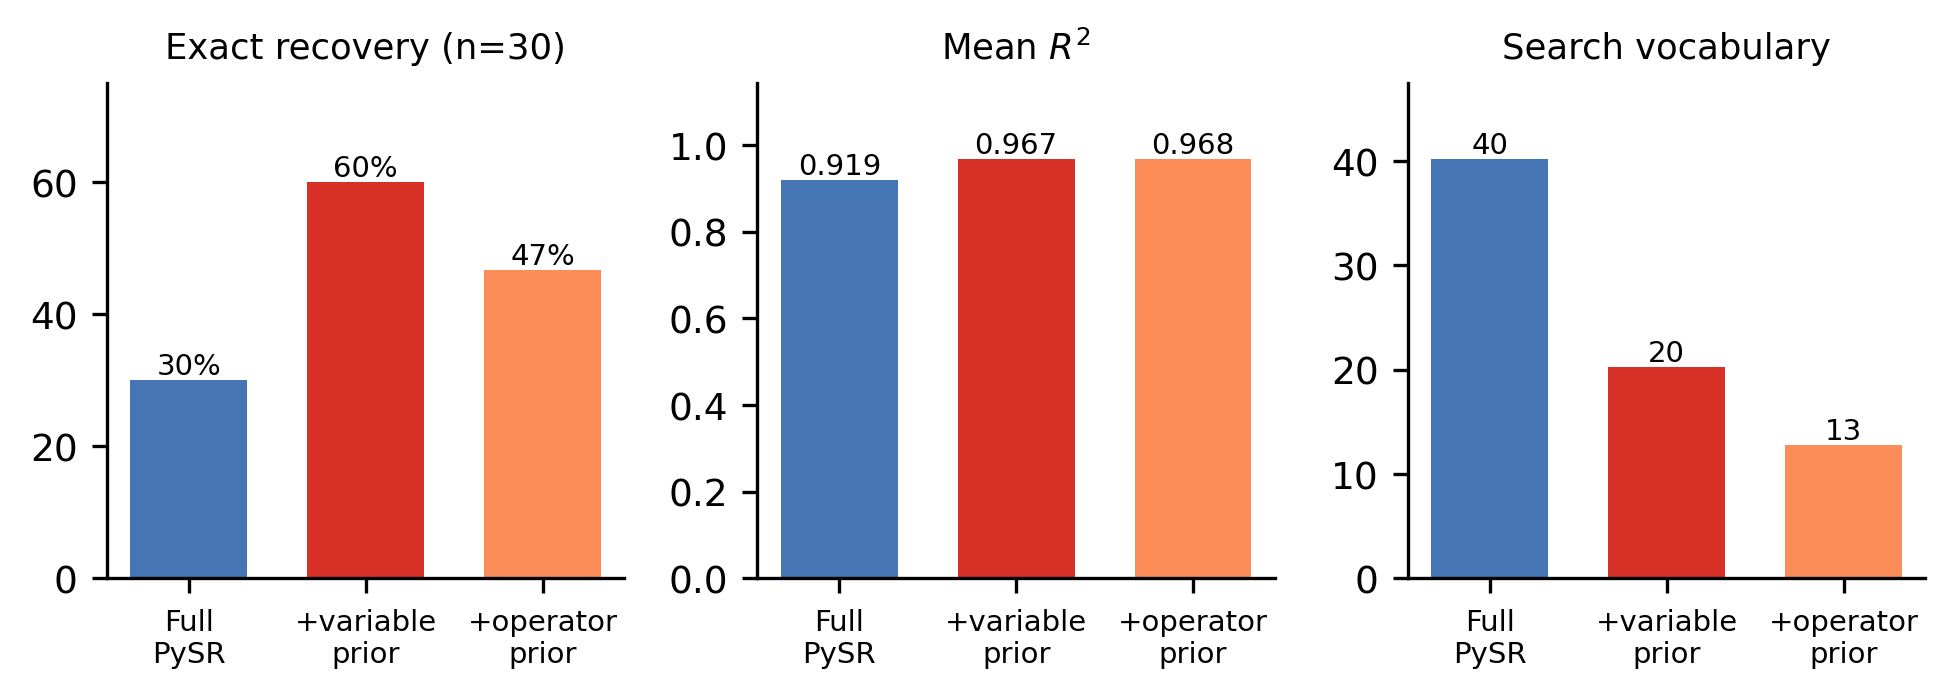
\includegraphics[width=0.95\linewidth]{figures/fig3_pysr_recovery.png}
\caption{\textbf{A variable prior makes a fixed-budget solver much stronger.}
Full PySR vs.\ $+$variable prior vs.\ $+$operator prior on a $30$-equation Feynman
subset ($10$\,s budget, $\sim\!20$ distractors). The variable prior doubles exact
recovery ($30\%\!\to\!60\%$), raises mean $R^2$ ($0.919\!\to\!0.967$) and halves
the search vocabulary ($40\!\to\!20$); adding the operator prior cuts the
vocabulary further but does not improve exact recovery.}
\label{fig:pysr}
\end{figure}

\begin{figure}[h]\centering
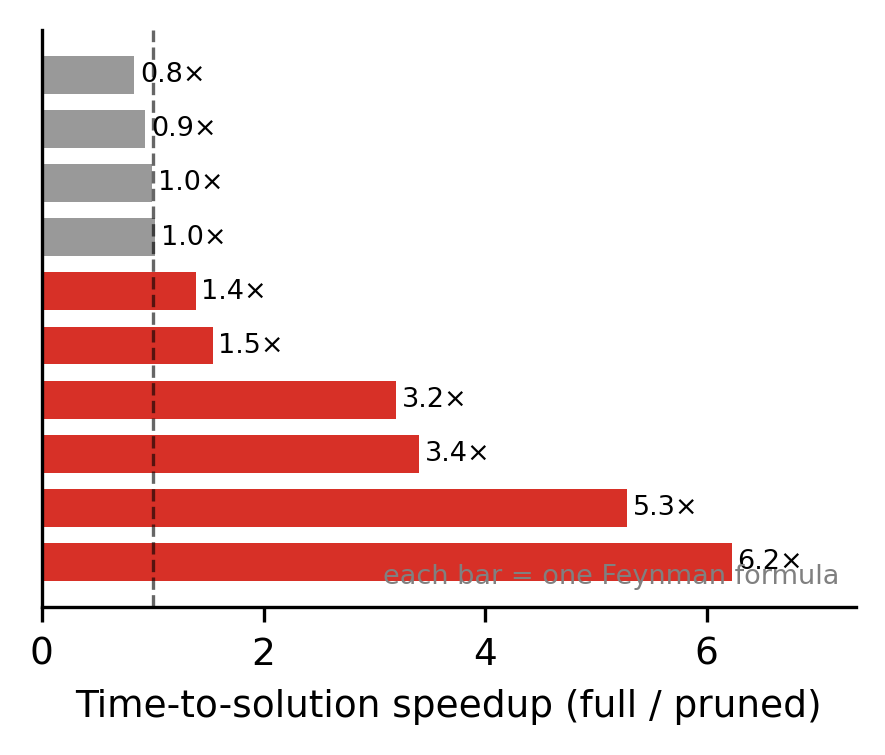
\includegraphics[width=0.55\linewidth]{figures/fig4_speed.png}
\caption{\textbf{Pruning the search space accelerates time-to-solution.}
Per-formula speedup (full search time divided by pruned-search time) with early
stopping on exact recovery. Typical physics formulas solve $3$--$6\times$ faster;
deep-tree formulas (depth-, not variable-limited) show little gain.}
\label{fig:speed}
\end{figure}

\begin{figure}[h]\centering
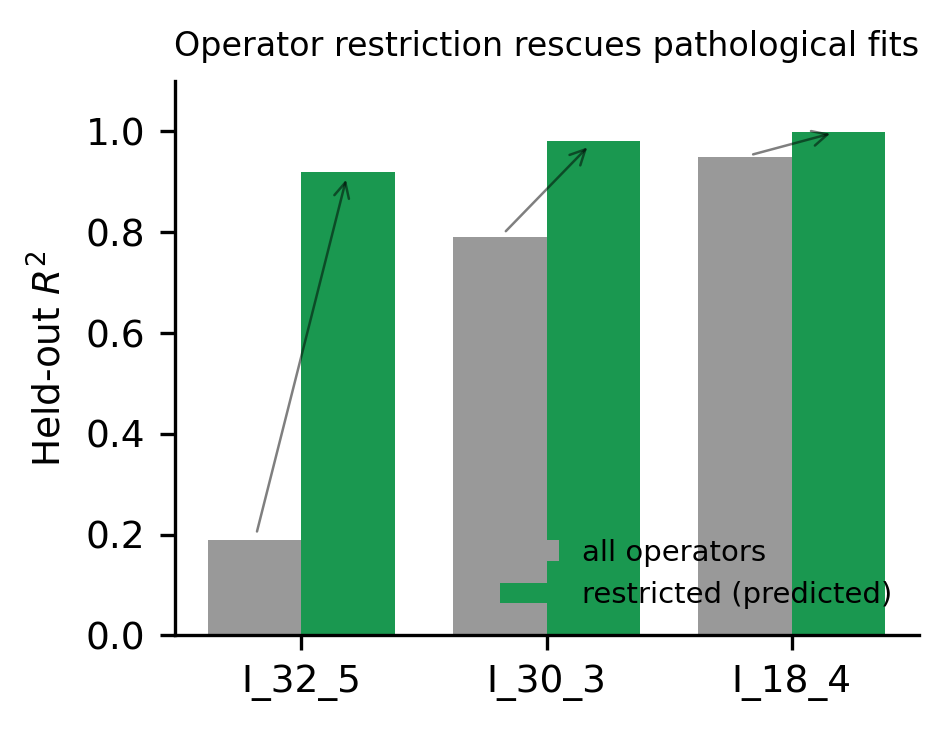
\includegraphics[width=0.5\linewidth]{figures/fig5_operator_safeguard.png}
\caption{\textbf{Operator restriction rescues pathological fits.} For cases where
full-operator search returns a spurious high-$R^2$ solution using exotic
operators, restricting the library to the predicted operators recovers a sane fit
(held-out $R^2$ before vs.\ after restriction). Operator priors are net-neutral on
average but valuable as an adaptive safeguard.}
\label{fig:op}
\end{figure}

\end{document}
